\documentclass[a2paper, 12pt]{article}
\usepackage[font={huge, bf}]{caption}
\usepackage{fontspec}
\setmainfont{Arial}
\usepackage{subcaption}
\usepackage{graphicx}
\usepackage{tikz}
\usepackage{tikzsymbols}
\usetikzlibrary{calc,patterns,shapes.geometric}
\usepackage{float}
\usepackage{pdflscape}
\usepackage{geometry}
\geometry{landscape, margin=2cm}
\captionsetup[subfigure]{justification=justified,singlelinecheck=false}
\pagestyle{empty}

\def\centerarc[#1](#2)(#3:#4:#5){\draw[#1] ($(#2)+({#5*cos(#3)},{#5*sin(#3)})$) arc (#3:#4:#5);}

\begin{document}
	\vspace*{\fill}
	\begin{figure}[!htbp]
		\centering
		\begin{subfigure}[b]{0.48\textwidth}
			\caption{Figure 1}
			\centering
			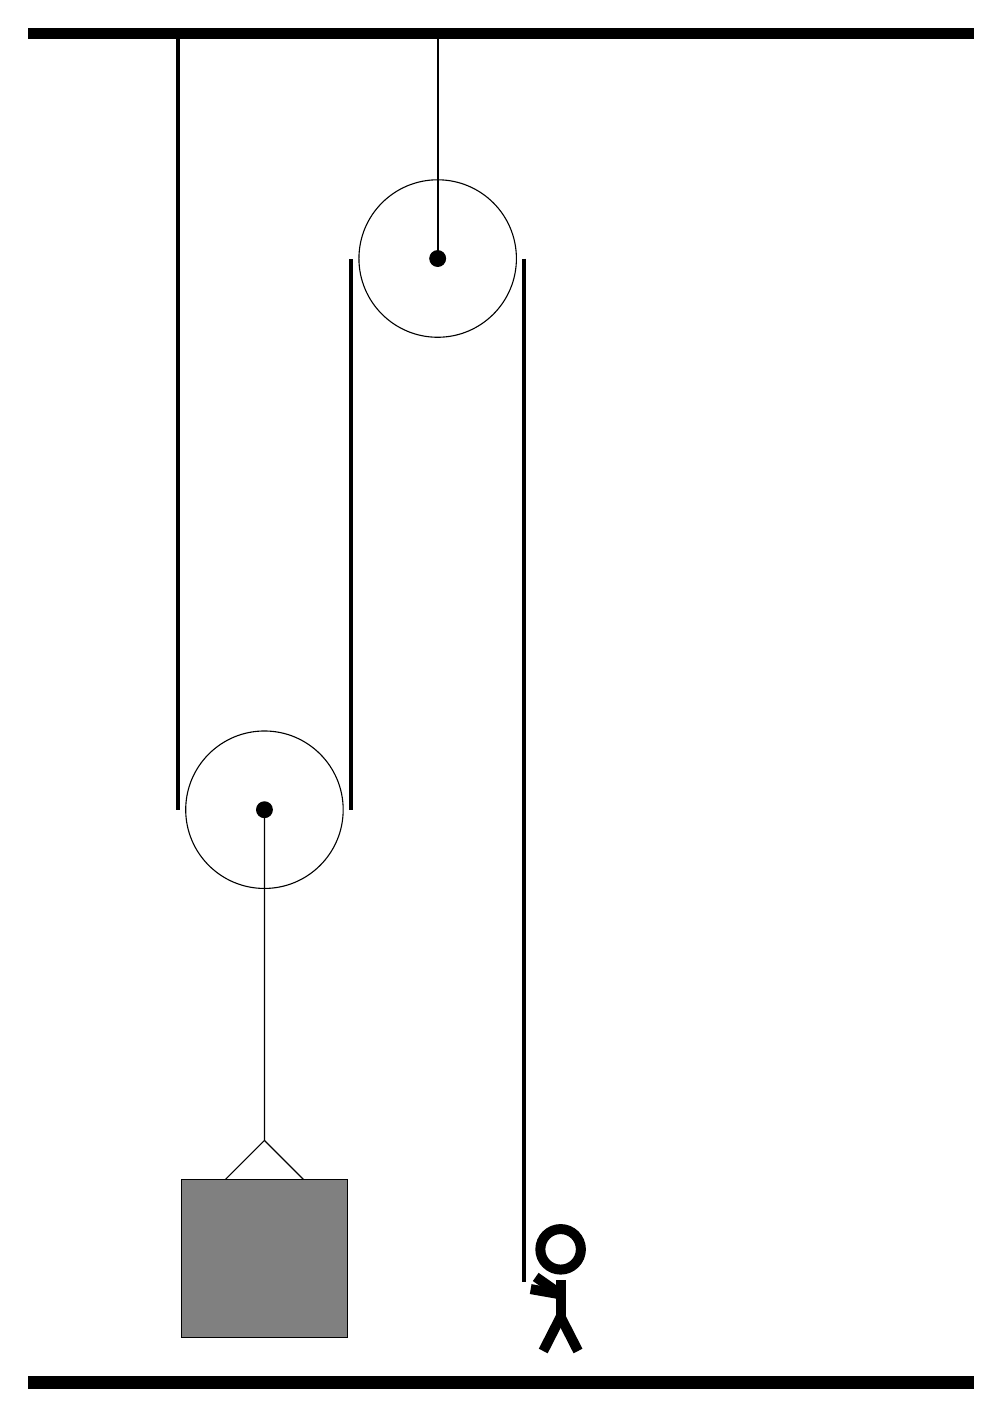
\begin{tikzpicture}
				\draw[fill=black] (-2, 14) rectangle (10, 14.125);
				
				\draw (3.2, 11.2) circle (1);
				\draw[fill=black] (3.2, 11.2) circle (0.1);
				\draw[thick] (3.2, 11.2) -- (3.2, 14);
				
				\draw (1, 4.2) circle (1);
				\draw[fill=black] (1, 4.2) circle (0.1);
				
				\draw (1, 4.2) -- (1, 0) -- (0.5, -0.5);
				\draw (1, 0) -- (1.5, -0.5);
				\draw[fill=black!50] (-0.05, -0.5) rectangle (2.05, -2.5);
				
				\draw[line width=0.5mm] (-0.1, 14) -- (-0.1, 4.2);
				\centerarc[line width=0.5mm](1, 4.2)(180:360:1.1);
				\draw[line width=0.5mm](2.1, 4.2) -- (2.1, 11.2);
				\centerarc[line width=0.5mm](3.2, 11.2)(0:180:1.1);
				\draw[line width=0.5mm](4.3, 11.2) -- (4.3, -1.8);
				
				\node at (4.7, -1.9) {\scriptsize \Strichmaxerl[10][-35][170]};
				
				\draw[fill=black] (-2, -3) rectangle (10, -3.15);
			\end{tikzpicture}
		\end{subfigure}
		\hfill
		\begin{subfigure}[b]{0.48\textwidth}
			\caption{Figure 2}
			\centering
			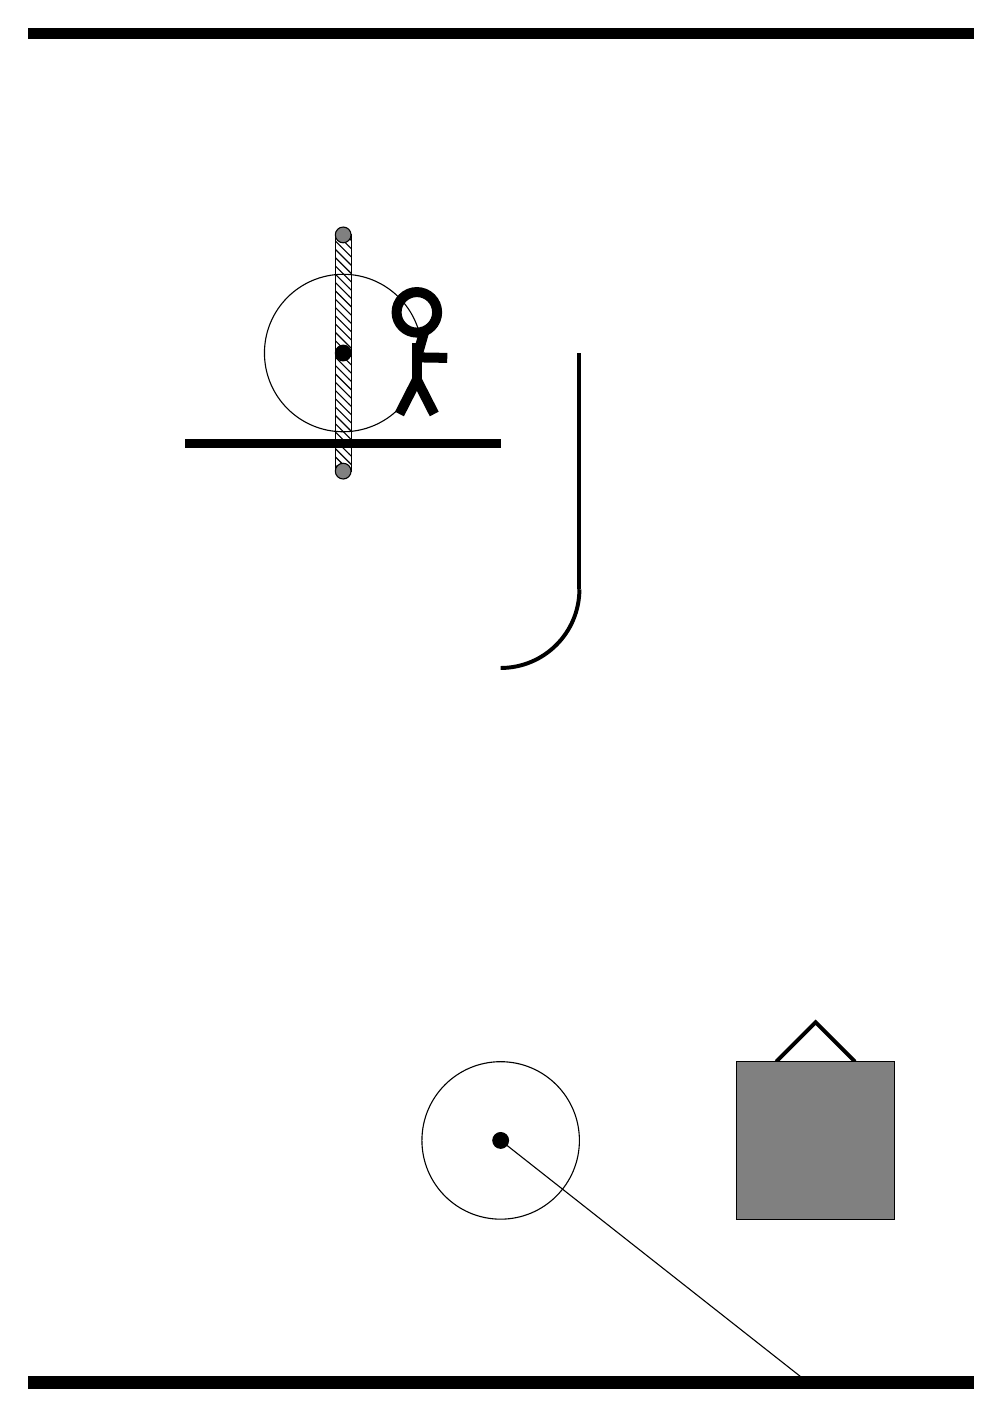
\begin{tikzpicture}
				\draw[fill=black] (-2, 14) rectangle (10, 14.125);
				
				\draw (4,0) circle (1);
				\draw[fill=black] (4,0) circle (0.1);
				\draw (8,-3.15) -- (4,0);
				
				\draw (2,10) circle (1);
				\draw[fill=black] (2,10) circle (0.1);
				\draw[pattern=north west lines, pattern color=black] (1.9,11.5) rectangle (2.1,8.5);
				\draw[fill=black!50] (2,11.5) circle (0.1);
				\draw[fill=black!50] (2,8.5) circle (0.1);
				
				\draw[line width=0.5mm](7.5,1) --  (8,1.5) -- (8.5,1);
				\draw[fill=black!50] (7, 1) rectangle (9, -1);
				
				\draw[line width = 0.5mm] (4,6) arc (270:360:1);
				\draw[line width = 0.5mm] (5,7) -- (5,10);
				
				\node at (3, 10) {\scriptsize \Strichmaxerl[10][-106][-1]};
				\draw[fill=black] (0, 8.9) rectangle (4, 8.8);
				
				\draw[fill=black] (-2, -3) rectangle (10, -3.15);
			\end{tikzpicture}
		\end{subfigure}
	\end{figure}
		\vspace*{\fill}
\end{document}